\documentclass[tikz,border=4pt]{standalone}
\usetikzlibrary{positioning, calc, decorations.pathreplacing}

\definecolor{def}{RGB}{73, 127, 170}
\definecolor{unused}{RGB}{40, 40, 40}
\definecolor{other}{RGB}{83, 83, 85}

\definecolor{pair0}{RGB}{100, 130, 150}
\definecolor{pair1}{RGB}{90, 105, 135} 
\definecolor{pair2}{RGB}{85, 80, 115}    
\definecolor{pair3}{RGB}{80, 55, 90}

%\nopagecolor
%\pagecolor{black!90} 

\begin{document}
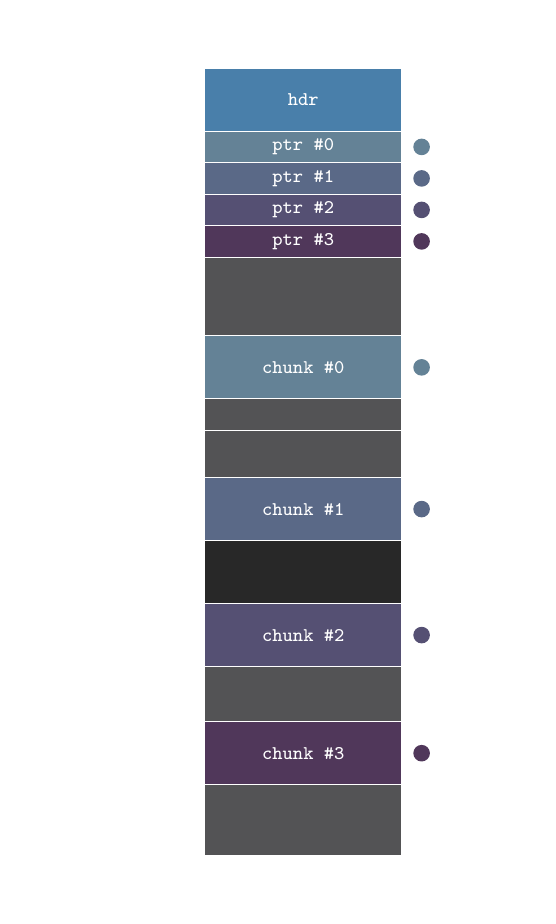
\begin{tikzpicture}[
    cell/.style={
        draw=white, 
        text=white,
        minimum width=2.5cm, 
        font=\scriptsize\ttfamily, 
        inner sep=0pt,
        outer sep=0pt,
        node distance=0pt
    },  
    info/.style={text=white, font=\scriptsize\ttfamily},    
    hdr_style/.style={cell, minimum height=0.8cm, fill=def},
    ptr_style/.style={cell, minimum height=0.4cm}, 
    chunk_style/.style={cell, minimum height=0.8cm}, 
    other_style/.style={cell, fill=other}, 
    unused_style/.style={cell, minimum height=0.8cm, fill=unused},
    tag_style/.style={
        draw=white,          
        thick,
        text=white,          
        fill=none,           
        font=\tiny\ttfamily\bfseries, 
        inner sep=2pt, 
        rounded corners=2pt
    },
    dot_style/.style={
        circle,
        draw=none, 
        inner sep=0pt,
        minimum size=6pt
    }
]

\node[hdr_style] (hdr) at (0,0) {hdr};

\draw[white] (hdr.north west) -- ++(0, 0.2cm);
\draw[white, dotted, thick] ([yshift=0.2cm]hdr.north west) -- ++(0, 0.3cm);

\draw[white] (hdr.north east) -- ++(0, 0.2cm);
\draw[white, dotted, thick] ([yshift=0.2cm]hdr.north east) -- ++(0, 0.3cm);

\node[ptr_style, fill=pair0, below=of hdr] (p0) {ptr \#0};
\node[ptr_style, fill=pair1, below=of p0] (p1) {ptr \#1};
\node[ptr_style, fill=pair2, below=of p1] (p2) {ptr \#2};
\node[ptr_style, fill=pair3, below=of p2] (p3) {ptr \#3};

\draw[decorate, decoration={brace, amplitude=3pt}, white] 
    ([xshift=-3pt]p3.south west) -- ([xshift=-3pt]p0.north west) 
    node[midway, left=8pt, info, align=right] {Pointer\\Table};
    
\node[other_style, below=of p3, minimum height=1.0cm] (m0) {};
\node[chunk_style, fill=pair0, below=of m0] (c0) {chunk \#0};
\node[other_style, below=of c0, minimum height=0.4cm] (m1) {};
\node[other_style, below=of m1, minimum height=0.6cm] (m2) {};
\node[chunk_style, fill=pair1, below=of m2] (c1) {chunk \#1};
\node[unused_style, below=of c1] (u0) {};
\node[chunk_style, fill=pair2, below=of u0] (c2) {chunk \#2};
\node[other_style, below=of c2, minimum height=0.7cm] (m3) {};
\node[chunk_style, fill=pair3, below=of m3] (c3) {chunk \#3};
\node[other_style, below=of c3, minimum height=0.9cm] (m4) {};

\draw[white] (m4.south west) -- ++(0, -0.2cm);
\draw[white, dotted, thick] ([yshift=-0.2cm]m4.south west) -- ++(0, -0.3cm);

\draw[white] (m4.south east) -- ++(0, -0.2cm);
\draw[white, dotted, thick] ([yshift=-0.2cm]m4.south east) -- ++(0, -0.3cm);

\node[dot_style, fill=pair0, right=4pt of p0] {};
\node[dot_style, fill=pair1, right=4pt of p1] {};
\node[dot_style, fill=pair2, right=4pt of p2] {};
\node[dot_style, fill=pair3, right=4pt of p3] {};

\node[dot_style, fill=pair0, right=4pt of c0] {};
\node[dot_style, fill=pair1, right=4pt of c1] {};
\node[dot_style, fill=pair2, right=4pt of c2] {};
\node[dot_style, fill=pair3, right=4pt of c3] {};

\path (c0.east) -- ++(1.6cm, 0);
\path (c0.west) -- (-3.5cm, 0);

\end{tikzpicture}
\end{document}